\subsubsection{Unstructured meshes}\label{unstructured-meshes}
In the scientific and high performance communities concurrent operations on
different meshes are commonly used; meshes can be used as discretisations to
numerically solve partial differential equations (PDEs). Usually these
simulations require millions of elements to get correct results. Structurally,
we can differentiate between structured and unstructured meshes.\\
Structured meshes are defined by blocks. Inside the blocks we have elements and
implicit connectivity between them. The blocks are organized in a structured
manner meaning that for every element in a block we can get all the neighboring
elements simply from indexing arithmetic without any further information.
Structured applications consist of loops over blocks which access datasets
defined on blocks and the access patterns required for an element is described
by stencils. A part of a block and a stencil describing access shown in Figure
\ref{fig:structured}. Most operations on structured grids can be easily
parallelised even on GPUs since all nodes can be processed simultaneously.

\begin{figure}
\centering
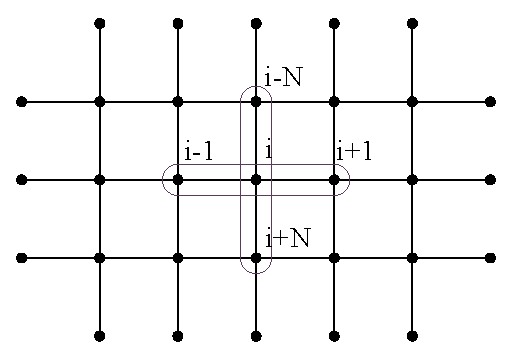
\includegraphics[width=4cm]{fig/svg/structured.eps}
\caption{Structured mesh and stencil describing access pattern}
\label{fig:structured}
\end{figure}

Unstructured meshes are defined by sets (e.g. nodes, edges, faces...), data
defined on the sets, and explicit connectivity information between sets
(mapping tables). For determining the neighbours of a set element the index
isn't enough, we need external information. Thus there is an overhead
associated with the reading of the mapping tables to determine the neighboring
elements, but we gain significant performance when we need finer resolution for
interesting parts of the mesh while a rougher resolution is sufficient for the
most of the mesh (e.g. in the case of PDE-s where the gradient changes slowly).
In such a case with structured meshes we need to compute unnecessary points
otherwise we wouldn't get correct results in areas where detail is necessary.

For unstructured meshes the computations on the mesh are given as operations on
sets. Basically a loop over the elements of a set, executing the same
operations for every element, while accessing data directly on the iteration
set or indirectly through a mapping. An example for a mesh and a mapping from
edges to cells are shown in Figure \ref{fig:unstructured}. For kernels that
only access data directly or only read data indirectly but write the data on
the iteration set, the whole iteration space could run simultaneously. However,
for kernels which indirectly increment data, we need to ensure that there are
no race conditions during the execution.

The parallelisation of such unstructured mesh operations is much harder than
for structured mesh codes: where the elements are writing data indirectly we
can not tell which elements could be computed at the same time from compile
time information, as it is driven by the mapping table. One of the most
commonly used approaches is to use a runtime colouring of elements to
parallelise the computation.  

\begin{figure}
\centering
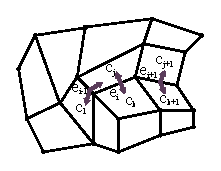
\includegraphics[width=4cm]{fig/svg/unstructured.eps}
\caption{Unstructured mesh, the arrow represents the mapping tells $e_i$ is
  connected to $c_j$ and $c_k$.}
\label{fig:unstructured}
\end{figure}

In our case the sets are represented as consecutive indexes from zero to the
size of the set. The mapping between two sets are represented as a mapping
table, an array which stores the index of set elements in the second set of the
mapping (referred as to-set) for every set element of the first set (from-set).
For the example in Figure \ref{fig:unstructured} a part of the mapping from
edges to cells is shown in Figure \ref{fig:mapping}. In this way we can access
the index of those elements which are connected to the current element of the
from-set from other sets (the to-sets of the mappings).

\begin{figure}
\centering
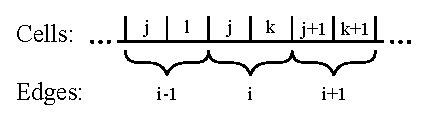
\includegraphics[width=6cm]{fig/svg/mapping.eps}
\caption{A part of the mapping from edges to cells.}
\label{fig:mapping}
\end{figure}

In our case we used some restrictions for the applications, but out work is
general enough that we are able to represent most applications in a way that
doesn't violate our restrictions. The first is that there is no data access
through multiple mappings. This means every data that we access is either
accessed directly with the index of the set we iterate on or it is accessed
with an index from one of to-sets of the accessible mappings get with using the
index of the current element. This restriction does not exclude applications
using nested indirections, since we can create a mapping that contains the
indexes that we access through multiple mapping. The second restriction is that
the result of the operations on the sets are independent from the order of
processing the elements of the sets. This restriction is necessary to ensure
that we can parallelise the operations, because there is no guarantee for
execution order in the parallelised versions.

